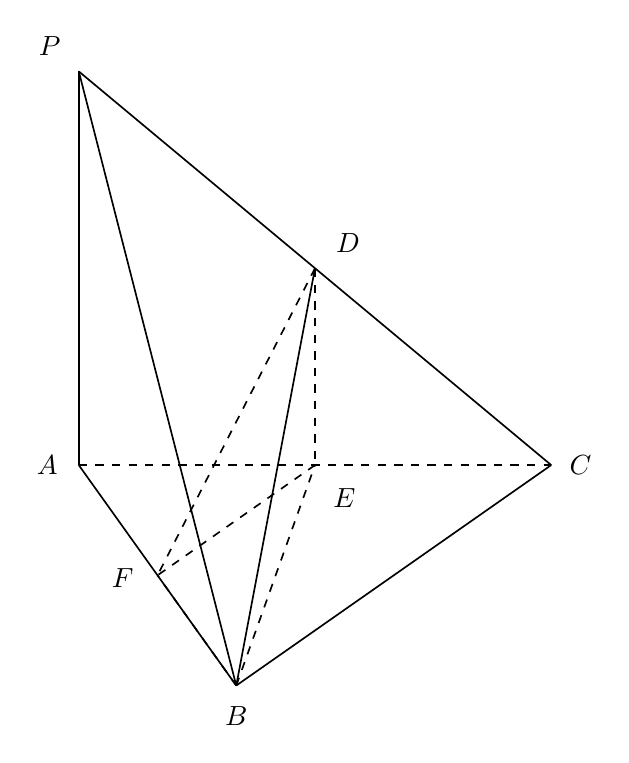
\begin{tikzpicture}[x=1cm,y=1cm,line width=0.6pt]
\coordinate (P) at (0,8);
\coordinate (A) at (0,3);
\coordinate (C) at (6,3);
\coordinate (B) at (2,0.2);
\coordinate (E) at (3,3);
\coordinate (F) at (1,1.6);
\coordinate (D) at (3,5.5);
% tetrahedron outline
\draw (P) -- (A);
\draw (P) -- (B);
\draw (P) -- (C);
\draw (A) -- (B);
\draw (B) -- (C);
\draw[dashed] (A) -- (C);
% mid-segment and auxiliary lines visible in original
\draw (B) -- (D);
\draw[dashed] (D) -- (F);
\draw[dashed] (D) -- (E);
\draw[dashed] (E) -- (F);
\draw[dashed] (B) -- (E);
\draw[dashed] (B) -- (F);
% labels with clearance
\node[above left,xshift=-3pt,yshift=2pt] at (P) {$P$};
\node[left,xshift=-4pt] at (A) {$A$};
\node[right,xshift=3pt] at (C) {$C$};
\node[below,xshift=0pt,yshift=-4pt] at (B) {$B$};
\node[above right,xshift=4pt,yshift=2pt] at (D) {$D$};
\node[below right,xshift=3pt,yshift=-5pt] at (E) {$E$};
\node[left,xshift=-5pt,yshift=-1pt] at (F) {$F$};
\end{tikzpicture}
